
\documentclass[11pt]{article}

\usepackage{common}
\usepackage{hyperref}
\title{HW1: Text Classification}
\author{Akhil Ketkar \\ akhilketkar@g.harvard.edu \\ \url{https://github.com/akhilketkar/CS287_HW1}}

\begin{document}
\maketitle{}

\section{Introduction}

The objective of this assignment is to classify text into categories. For
instance, we might be given a movie review and asked to predict the rating
that the movie was given by the reviewer. Other examples might be classifying
an email as spam or not spam. Alternatively classifying it as
important or not important as GMail now does. We use 3 linear models from
\citep{murphy2012machine} for this assignment.

\section{Problem Description}

\begin{itemize}
  \item \textbf{Input Representation}: We represent the input text using some set of features
  $\mcF$. Each data point is represented by a vector $\boldx$ of size
  $d_{in} = |\mcF|$ where $x_{f_i} = 1$ if that feature is "on" and 0 otherwise.
  In practice we use a sparse representation to store $\boldx$ since most of
  it's entries are 0.

  \item \textbf{Output Representation}: The output categories are elements of a set
  $\mcC$ where $d_{out} = |\mcC|$
  and are represented by one-hot vectors $\boldy \in \{0,1\}^{d_{out}}$ where
  $y_i = 1$ if the piece of text is in category $i \in \mcC$.

  \item \textbf{Learning Representation}:  So the goal is to learn a function
  $\bold{\hat{y}} = f(\boldx)$ that maps the
  feature based representation of the text to a score vector $\bold{\hat{y}}$. The
  highest scoring class is our prediction of the output.
  $\hat{c} = \argmax_{i \in \mcC} \hat{y}_i$

  \item \textbf{Evaluation}: We measure how well the algorithm performs by simply
  counting the percentage
  of time we get the right answer. $\sum_{i=1}^N \frac{\bold1(y_i = \hat{c})}{N}$

\end{itemize}

\section{Model and Algorithms}

For all the models below (unless mentioned otherwise) we use bag of words
features. i.e $d_{in}$ is the number of unique words in all the text samples.
Thus each piece of text is represented simply by turning "on" the feature
corresponding to each unique word in the text.

The models we use are also all linear. i.e The functions we will try to learn
will be of the form $\bold{\hat{y}} = f(\boldx \boldW + \boldb)$ where $\boldW,\boldb$
are the parameters. In each model we will define a loss function that will
capture some notion of doing badly at the given task (text classification in
this case). We will then perform a straightforward minimization of the loss
function. The "learning" will be the set of parameters that produce the minima.

\begin{itemize}
  \item \textbf{Multinomial Naive Bayes}
  In this model we assume that the features are conditionally independent of each
  other given $\boldy_i$ and the parameters. We also assume that the features are
  generated from a multinomial distribution. The loss function $L$ we use here is the
  negative joint log-likelihood.

  $$L(\boldW,\boldb) = - \sum_{i=1}^N \log p(\boldx_i,\boldy_i | \boldW,\boldb)$$

  Using the chain rule we can simplify the RHS into a marginal and a conditional.
  Independence further simplifies the expression giving

  $$L(\boldW,\boldb) = - \sum_{i=1}^N \log \prod_{j=1}^{d_{in}}
    p(x_{f_i} = 1| \boldy_i, \boldW, \boldb) p(\boldy)$$

  We can find best estimates for both the terms in the above expression in closed
  form by simply counting how often a feature appears in a particular category
  and by counting the number of times a category is seen in the dataset.

  \item \textbf{Multinomial Logistic Regression}

  In this model we take a discriminative approach and estimate $p(\boldy|\boldx)$
  directly by using the softmax function which takes in any real vector and turns
  it into probabilities (each value in (0,1) and the sum = 1).
  $$ p(\bold{\hat{y}}|\boldx) = softmax(\boldx \boldW + \boldb) $$

  Then we use a cross-entropy loss function to compute how badly our probabilities
  differed from the actual.
  $$ L(\boldW, \boldb) = \sum_{i=1}^{N} L_{cr}(\bold{\hat{y}_i},\boldy_i) $$
  where
  $$ L_{cr}(\bold{\hat{y}},\boldy) = - \sum_{j=1}^{d_{out}} y_j \log \hat{y}_j $$

  Given that $\boldy$ is a one-hot vector this simplifies to a single term. If
  we try to optimize this loss, the weights will blow up to infinity so we add a
  $l_2$ regularization term. There is no closed form solution to this optimization
  so we have to use some form of gradient decent. Here we've used mini-batch
  stochastic gradient decent.

  \item \textbf{Linear SVM}

  In this model we remove the probabalistic interpretation of
  $\bold{\hat{y}} = \boldx \boldW + \boldb$ and simply treat it as a score.

  We then use the hinge loss function to compute the loss of our score.
  $$ L(\boldW, \boldb) = \sum_{i=1}^{N} L_{h}(\bold{\hat{y}_i},\boldy_i) $$
  and

  $$ L_h(\bold{\hat{y}},\boldy) = \max \{0,1 - (\hat{y}_c - \hat{y}_{c'}) \}$$

  where $c$ is the true class i.e $y_c = 1$ and $c'$ is the class to which
  we assigned the highest score that was not the true class i.e
  $c' = argmax_{d \in \mcC \setminus \{c\}} \hat{y}_d$

  We add a regularization term similar to the one in logistic regression to this
  loss function as well so that we penalize large weights.

\end{itemize}

\section{Experiments}

\begin{itemize}
    \item \textbf{Naive Bayes}

    Since the optimization for this model has a closed form result and there's
    only one hyperparameter to tune, we can afford to a grid search over $\alpha$
    using the validation set. That results in the figure shown below in
    Figure~\ref{fig:nbA}.

    The accuracy achieved using this model is in the low to mid 30s.

    \item \textbf{Logistic Regression}

    This is a relatively expensive model to train. With a batch size of 100 and
    number of epochs set to 1000, the model takes ~120 seconds to train. It is not
    feasible in moderate The loss function from a sample run is shown below in
    Figure~\ref{fig:lLR}. This model however tuned properly seems to give the best
    performance.

    In terms of selecting hyperparameters (weight decay $\lambda$, learning rate
    $\eta$ and size of mini-batch $M$) I experimented with a few values and
    selected what seemed to work best on the validation set. The value of the loss
    seems to oscillate quite a bit as can be seen from the previous figure. Given
    this behavior, we can infer that the model is being pushed too far in each step
    so a smaller learning rate should be used. It probably also calls for a larger
    weight decay rate.

    \item \textbf{Linear SVM}

    This model is less expensive to train but performs worse than Logistic
    Regression. With a batch size of 100 and number of epochs set to 1000, the
    model takes ~90 seconds to train.The loss function from a sample run is shown
    below in Figure~\ref{fig:lSVM}.

    The graph of the training loss for this model looks similar to the training
    loss for Logistic Regression. I chose hyperparameters in a similar fashion
    to that model (by trial and error).
\end{itemize}

\begin{figure}
  \centering
  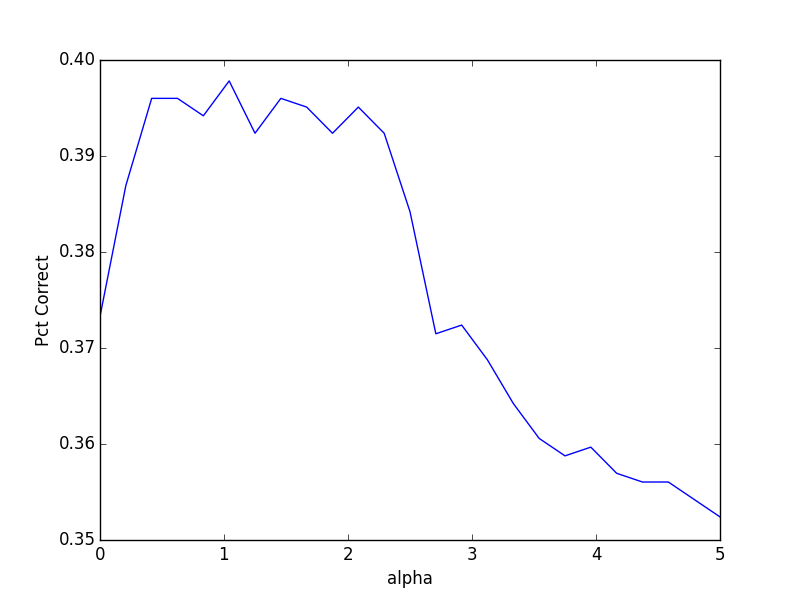
\includegraphics[width=0.5\textwidth]{nbAlphaGS}
  \caption{\label{fig:nbA} Grid Search over $\alpha$}
\end{figure}

\begin{figure}
  \centering
  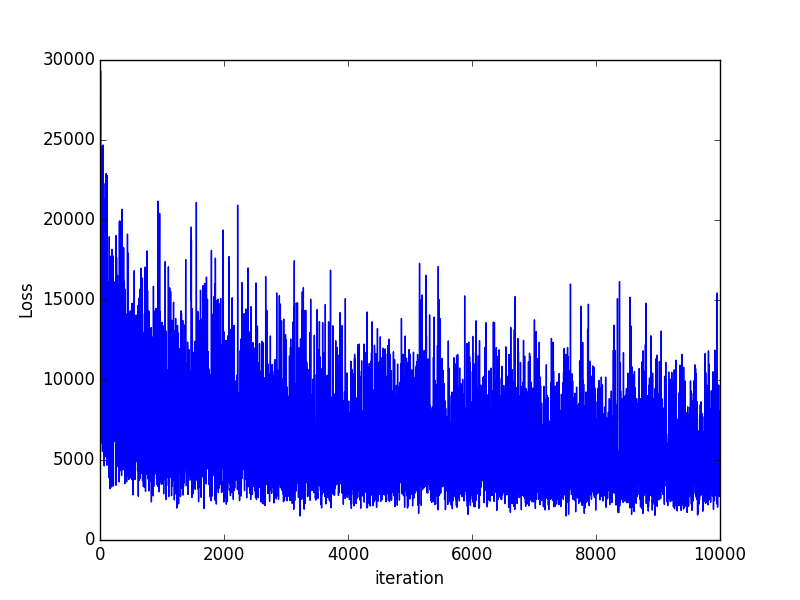
\includegraphics[width=0.5\textwidth]{lossLR}
  \caption{\label{fig:lLR} Training Loss for LR}
\end{figure}

\begin{figure}
  \centering
  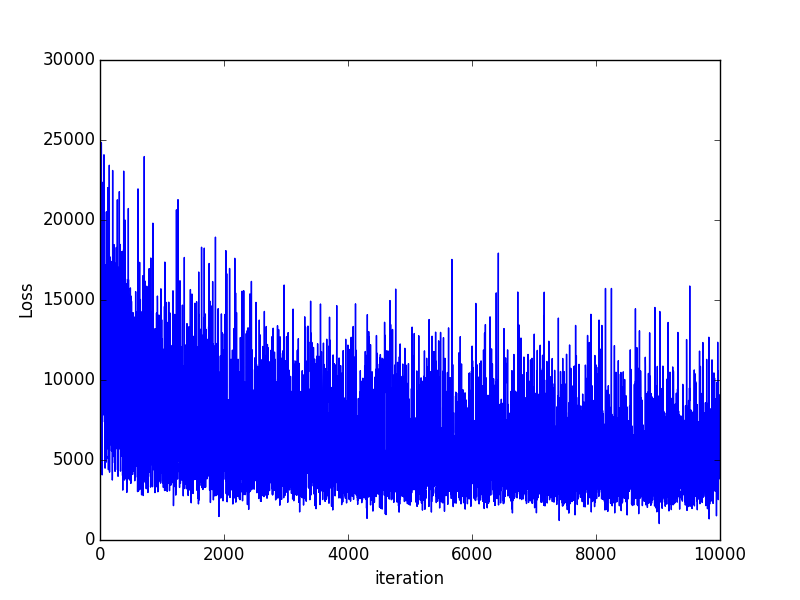
\includegraphics[width=0.5\textwidth]{lossSVM}
  \caption{\label{fig:lSVM} Training Loss for SVM}
\end{figure}


The baseline for all these models should be 0.2 since thats the score we would
get if we assigned labels at random.

\begin{table}[h]
\centering
\begin{tabular}{llr}
 \toprule
 Model &  & Acc. \\
 \midrule
 \textsc{Baseline 1} & & 0.20\\
 \textsc{Model 1: NB} & & 0.36 \\
 \textsc{Model 2: LG} & & 0.41719 \\
 \textsc{Model 3: SVM} & & 0.37\\
 \bottomrule
\end{tabular}
\caption{\label{tab:results} Table with the main results.}
\end{table}

\section{Conclusion}

Some progress has been made over random assignment, but accuracy of high 30s to
low 40s is still quite poor. A lot of progress can be made on this models.

Potential improvements:

\begin{itemize}
  \item Better Features:
  We're ignoring the structure inherent in the data. Not taking into account
  qualifying terms like "but", "not" etc.

  \item Faster Processors:
  This will allow faster training and experimentation with hyperparameters.

  \item Better Model:
  All these models are linear in the features which can certainly be improved
\end{itemize}

\bibliographystyle{apalike}
\bibliography{writeup}

\end{document}

%Settings used for LR: th HW1.lua -datafile SST1.hdf5 -classifier lr -M 100 -N 10000 -eta 0.05 -lambda 0.8
